\documentclass[11pt,a4paper]{article}
\usepackage[T1]{fontenc}
\usepackage{lmodern,microtype,amsmath,amssymb,booktabs,tabularx,array}
\usepackage[margin=22mm]{geometry}
\usepackage{xcolor,tikz,hyperref}
\usetikzlibrary{positioning,arrows.meta}
\definecolor{navy}{HTML}{193B54}
\hypersetup{colorlinks=true,linkcolor=navy,urlcolor=navy,
pdftitle={Tensor temporal encoders: architectures and exploratory screen}}
\setlength{\parindent}{0pt}
\setlength{\parskip}{6pt}
\newcolumntype{Y}{>{\raggedright\arraybackslash}X}
\newcommand{\code}[1]{{\small\nolinkurl{#1}}}
\begin{document}
{\LARGE\bfseries\color{navy} Tensor temporal encoders}\par
{\large Returning to the tensor proposal without an EEGNet front end}\par
Research branch: \code{research/baseline-accuracy}. Study designed 4 October 2026.

\section{Question and evidence boundary}
Can a tensor representation extract useful temporal features directly from EEG,
instead of relying on EEGNet's temporal and spatial convolutions? We implement
three tensor alternatives and two controls. All new encoders retain ordered
time patches and feed a compact temporal Transformer. The original proposal's
fixed time--frequency representation motivates the first option; the other two
learn multilinear projections from classification loss.

The previous study's compact EEGNet--Transformer achieved 64.87\% mean
validation balanced accuracy over nine participants and three seeds. That result
motivates retaining it as a reference, but this new screen reruns its seed-0
fits alongside the candidates. Only scores from the same new comparison should
be used to rank the new encoders.

\textbf{Friend's branch.} Revision \code{3c9a170} reports 56.15\% held-out
within-T-session test accuracy over nine participants and seed 0. Its README
explicitly excludes Signal Transformer from those results: the backbone is
EEGNet with electrode attention. Tucker completion is bypassed for full inputs,
so both completion and baseline variants have the same full-input predictions.
The branch reports completion gains of 3.10, 1.70 and $-0.06$ percentage points
at 16, 11 and 6 channels. These are collaborator-reported measurements;
underlying predictions and checkpoints are unavailable in the branch.
Its artifact inclusion, filtering context, 500-epoch training and validation-loss
selection differ from our protocol. Its test score and our validation score do
not establish a model ranking. See the
\href{https://github.com/georgiipr/agfl-inm/blob/3c9a170/README.md}{pinned branch README}.

\section{Shared inputs and temporal head}
Each participant is trained separately on BCI IV 2a: 22 EEG channels at 250 Hz,
four motor-imagery classes, four cue-aligned seconds per trial. We reuse the
verified historical approximately 60/20/20 T-session split and expose only
training and validation arrays to model fitting and scoring. Artifact-marked
trials are excluded. Filtering is 2--30 Hz within each one-second channel/window;
channel normalization uses training samples only.

The input is $X\in\mathbb{R}^{B\times22\times4\times250}$ with a Boolean
mask $M\in\{0,1\}^{B\times22\times4}$. Missing samples are selected to zero
with \code{torch.where} before arithmetic. Every window must contain an observed
electrode. Hidden NaNs must have exactly the same predictions as hidden zeros.

\begin{center}
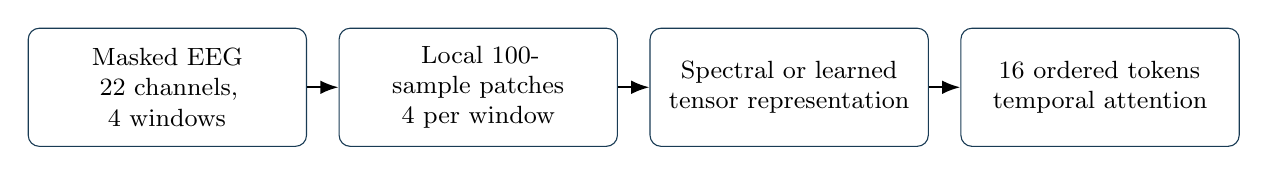
\begin{tikzpicture}[node distance=4mm,
box/.style={draw=navy,rounded corners,align=center,text width=33mm,
minimum height=15mm,font=\small},arr/.style={-{Latex},thick}]
\node[box] (x) {Masked EEG\\22 channels, 4 windows};
\node[box,right=of x] (p) {Local 100-sample patches\\4 per window};
\node[box,right=of p] (e) {Spectral or learned\\tensor representation};
\node[box,right=of e] (a) {16 ordered tokens\\temporal attention};
\draw[arr] (x)--(p);\draw[arr] (p)--(e);\draw[arr] (e)--(a);
\end{tikzpicture}
\end{center}

Patches begin at samples 0, 50, 100 and 150 of each 250-sample window. They cover
the whole window, overlap by 50 samples, and never cross a mask boundary.
There are 16 ordered patches per trial. The four new arms project their patch
representations to 32 features, add fixed sinusoidal time positions and a
learned projection of the 22 availability bits at that patch, and apply one
pre-LayerNorm Transformer layer: four heads, feed-forward width 64, GELU and
dropout 0.1. Final LayerNorm and mean temporal pooling produce 32 values;
appending the original 88 mask flags gives a linear four-class readout.

Latent channel components are feature coordinates inside each time token, not
separate attention tokens. This is a deliberate temporal-head adaptation of
the original component-by-window proposal. The reference retains its original
31 EEGNet-derived tokens and original mask-conditioned head.
Comparisons against that reference therefore test the complete architecture:
token count, preprocessing inside the encoder and mask conditioning also differ.
The raw tensor pair provides the narrower temporal-factorization comparison.

\section{Three tensor architecture options}
\subsection{A: spectral features and frozen Tucker inference}
\code{fixed_spectral_tucker} computes a periodic Hann-windowed FFT of each local
100-sample patch. With frequency spacing 2.5 Hz, bins 1--12 cover 2.5--30 Hz.
For each coefficient $z$, use
\[
 f=\log\!\left(\frac{|z|^2}{\sum_s h_s^2}+10^{-6}\right).
\]
Each channel/frequency feature is standardized with its training-only population
mean and standard deviation (floor $10^{-6}$). This gives
$F\in\mathbb{R}^{B\times22\times16\times12}$.

Training-only alternating reconstruction fitting learns factors
$U\in\mathbb{R}^{22\times4}$ and $V\in\mathbb{R}^{12\times4}$ for 30 epochs.
Both become frozen buffers. At every time patch, infer the core from observed
channels $O_t$:
\[
 G_t^*=\arg\min_G
 \frac{\|F_{O_t,t,:}-U_{O_t,:}GV^\top\|_F^2}{|O_t|\,12}
 +10^{-3}\|G\|_F^2.
\]
The inherited exact ridge solver uses float64; the ridge normal-equation scale
is $|O_t|\,12\,10^{-3}$. Flattening each $4\times4$ core gives 16 features per
time token before projection to 32. Classification trains the temporal head,
not the spectral transform or Tucker factors. This is the closest option to
the original proposal. Low reconstruction loss does not imply high accuracy.

\textbf{Matched-feature control:} \code{spectral_dense} uses the same spectral
features and standardization, but flattens 22 channels $\times$ 12 frequencies
and learns a dense $264\to16$ map before the same head. This compares complete
representations. Frozen versus supervised fitting and different parameter counts
mean that a score difference cannot be attributed solely to tensor structure.

\subsection{B: learned channel--time projection}
\code{dense_temporal_patch} learns a spatial factor
$U\in\mathbb{R}^{22\times4}$ and temporal basis $V\in\mathbb{R}^{100\times8}$:
\[
 H_{btrf}=\sum_{c,s}X^{\rm patch}_{bcts}U_{cr}V_{sf}.
\]
The $4\times8$ core is transformed elementwise by
$\log(H^2+10^{-6})$ to retain an energy-sensitive nonlinearity, then flattened
into 32 features per patch. All factors and the head learn from classification
loss. This is a supervised separable tensor projection, not reconstruction-fitted
Tucker inference. Missing channels are zero-filled and identified to the head;
there is no observed-entry inverse solve or guaranteed completion.

\subsection{C: factorized temporal-patch projection}
\code{learned_tensor_patch} reshapes a 100-sample patch into $10\times10$ and
constrains the temporal basis to factors $A\in\mathbb{R}^{10\times2}$ and
$D\in\mathbb{R}^{10\times4}$:
\[
 H_{btrij}=\sum_{c,a,z}X^{\rm patch}_{bctaz}U_{cr}A_{ai}D_{zj}.
\]
This again yields 32 core coordinates and uses the same energy nonlinearity
and temporal head as B. The $10\times10$ reshape is a parameter-sharing prior
on consecutive temporal samples, not a physical two-dimensional EEG geometry.
It replaces 800 temporal weights by 60, reducing temporal flexibility.
Factors have unit column norms after optimizer steps.

These learned operators replace the EEGNet stack, but are mathematically
separable linear filters on temporal patches followed by a power nonlinearity.
The tensor factorization specifies parameter sharing; the attention rule remains
standard multi-head attention.

B is the temporal-unfactorized control for C; it still has a factorized spatial
projection. Both start from the same spatial factor, temporal operator and head:
$V_{(a,z),(i,j)}=A_{ai}D_{zj}$. Thereafter B can leave that restricted temporal
family. This makes the comparison more informative than unrelated random starts,
although parameterization and optimization geometry necessarily differ.

\section{Loss, screening protocol and reproducibility}
All classifier arms use unweighted four-class cross-entropy:
\[
 \mathcal{L}_{\rm cls}=-\frac1N\sum_n
 \log\operatorname{softmax}(\ell_n)_{y_n}.
\]
AdamW uses learning rate $10^{-3}$, weight decay $10^{-4}$, batch size 32,
gradient norm clipping at 1, 10 warm-up epochs then cosine decay, and at most
250 epochs. Early stopping starts after 75 epochs with patience 50.
Selection uses full-input validation balanced accuracy, then lower validation
log loss, then the earlier epoch. There is no reconstruction term in classifier
training; architecture A has its separate training-only reconstruction stage.

The bounded screen has nine participants, seed 0 and five arms: 45 fits.
Training uses full inputs only. Secondary validation evaluation covers full
22 channels and static/dynamic random retention of 16 or 6 channels, with five
matched repeats for each degraded condition. Means average mask repeats before
participants equally. No test score is used for architecture or epoch selection.

The primary architecture contrast is C minus B. Secondary contrasts include
A minus the spectral dense control and each new arm minus the EEGNet--Transformer
reference. The prespecified exploratory screen requires at least two percentage
points mean balanced-accuracy gain and positive differences in at least six of
nine participants. Participant bootstrap intervals use 2,000 resamples and seed
20261004. One seed does not measure training-seed stability; repeated use of
validation for epoch and architecture selection makes these exploratory scores.
Independent session/dataset confirmation is required before strong generalization
claims. Multiple unadjusted comparisons do not establish statistical superiority.

Initialization, fitting randomness and data-order randomness are controlled.
Calibration sees training arrays only. Each selected checkpoint is reloaded and
its predictions verified. Saved source/configuration/package identities and
artifact checksums prevent incompatible reuse. New study outputs are isolated
from every completed study. Actual run coverage and measurements follow.

\textbf{CPU-thread audit.} This screen fixes one PyTorch CPU thread per fit.
The older real-data candidate runner used the environment default. A bounded
one-epoch diagnostic reproduced the new A01 reference exactly with one thread
and the historical reference exactly with eight threads. After full fitting,
A01 selected the same epoch and class predictions, with small probability
differences. Historical cross-thread bitwise equality is therefore not a
requirement; exact checkpoint replay within the new study is required.

\section{Measured results and verdict}
\IfFileExists{tensor_temporal_results.tex}{\textbf{Complete exploratory screen:} 45 fits, nine participants and seed 0.
All percentages below are participant-equal balanced accuracy on training or
validation data. No test-set performance is claimed.
\begin{center}
\begin{tabular}{@{}lrrrr@{}}\toprule
Model & Parameters & Train (\%) & Validation (\%) & Log loss \\ \midrule
EEGNet--Transformer & 11,092 & 74.69 & 63.71 & 1.029 \\
Spectral dense control & 14,580 & 78.73 & 50.97 & 1.435 \\
Spectral Tucker (A) & 10,340 & 65.17 & 45.47 & 1.625 \\
Channel--time tensor (B) & 11,740 & 76.53 & 44.21 & 1.680 \\
Factorized temporal (C) & 11,000 & 55.85 & 40.82 & 1.394 \\
\bottomrule\end{tabular}\end{center}
\textbf{Accuracy verdict.} Keep the EEGNet--Transformer reference for the
full-input classification goal. None of these concrete tensor versions, nor
the spectral dense control, passes the prespecified accuracy screen against it.
The frozen spectral Tucker model loses 18.24 percentage points to the reference.
This rejects these configurations as accuracy replacements under this protocol;
it does not establish that every tensor encoder is ineffective.
\begin{center}\begin{tabular}{@{}lrrr@{}}\toprule
Matched contrast & Gain (pp) & 95\% interval (pp) & Positive \\ \midrule
Factorized C minus B & -3.39 & [-6.63, -0.46] & 3/9 \\
Frozen A minus spectral dense & -5.50 & [-10.49, -0.87] & 2/9 \\
\bottomrule\end{tabular}\end{center}
The restricted temporal factorization saves 740 parameters but reduces accuracy
in the matched comparison. C has lower log loss than B (1.394 versus 1.680),
so the accuracy result should not be mistaken for uniformly worse probability
predictions. Neither raw tensor variant is a strong classifier in this screen.
\subsection*{Availability tradeoff}
\begin{center}
\begin{tabular}{@{}lrrrrr@{}}\toprule
Model & Full & Static 16 & Dynamic 16 & Static 6 & Dynamic 6 \\ \midrule
EEGNet--Transformer & 63.71 & 35.88 & 34.59 & 31.11 & 31.24 \\
Spectral dense control & 50.97 & 37.33 & 38.86 & 29.14 & 28.67 \\
Spectral Tucker (A) & 45.47 & 36.98 & 36.71 & 33.53 & 34.08 \\
Channel--time tensor (B) & 44.21 & 29.85 & 27.78 & 25.33 & 25.86 \\
Factorized temporal (C) & 40.82 & 29.58 & 28.24 & 24.98 & 25.36 \\
\bottomrule\end{tabular}\end{center}
Frozen spectral Tucker is worth retaining as a robustness hypothesis. With
six retained channels it exceeds the spectral dense control by 4.39 pp
(static; interval [0.64, 8.27], 7/9 positive) and 5.40 pp (dynamic;
[1.41, 10.58], 8/9 positive). Relative to EEGNet--Transformer, its corresponding
gains are 2.42 pp ([0.20, 4.72], 7/9) and 2.84 pp ([$-0.08$, 5.77], 6/9).
These secondary condition-specific intervals are unadjusted and exploratory.
The approximately 34\% severe-loss accuracy, single training seed and full-input
penalty do not establish a strong or generally superior robust classifier.
Frozen versus dense also changes supervision and capacity, so the difference
is not uniquely attributable to the tensor decomposition.
\newpage
\subsection*{Recommended next hypothesis, not a measured result}
Keep the local spectral representation and observed-entry ridge inference,
but test classification-driven fine-tuning of its factors through a
differentiable ridge solve. Initialize frozen and trainable variants from the
same fitted factors and use identical ranks, temporal head and training masks.
This would test whether reconstruction-only fitting discards label information
while preserving the original availability mechanism. It is an untested,
post-screen hypothesis; improvement is not guaranteed. Introducing mixed
22/16/6-channel training would require a separate matched training-regime study.
\subsection*{Evidence and checks}
The implementation passed 17 new model/runner tests and all 72 existing
encoder-candidate tests. Tests include hidden NaNs, temporal patch isolation,
training-only frozen calibration, matched initial tensor operators, optimizer
gradient paths, deterministic repeated fits, selection ties and corrupt-artifact
rejection. Synthetic loss reduction is a software check only.
All 45 selected checkpoints passed exact saved-prediction reload checks.
The independent audit passed for all nine participants. It rebuilt masks,
replayed all 945 validation-condition evaluations, and independently recomputed
participant averages and bootstrap contrasts. The saved audit accompanies the
machine-readable report.
Reports: \code{results/tensor-temporal-screen-v1/report/summary.json},
\code{scores.csv}, \code{robustness.csv}, \code{contrasts.csv}, and
\code{independent_audit.json}. The independent audit can be rerun with
\verb|.venv/bin/python scripts/audit_tensor_temporal_screen.py|.
Its output defaults to \code{/tmp/agfl-tensor-temporal-independent-audit.json}.
\par Study identity:\par
\code{6c3d8edc5a13eefbd378282d593165c2d8ec9a6c3f1fd6aa81655d75c7749a8f}.
\par
The cohort used four independent participant processes, each with one PyTorch
thread; per-fit wall time includes contention and is not a controlled speed benchmark.
}{
The real-data screen has not yet been completed. No accuracy is asserted here.}

\section{Originality and reproducible use}
Tucker decompositions and learned tensor-contraction layers are established
methods, not inventions of this study. The new code tests their integration
with local EEG patches, known availability and a temporal attention head.
An exact configuration being new to this repository is not evidence of
architectural novelty or state-of-the-art performance. Relevant primary sources
are \href{https://www.kolda.net/publication/koba09/}{Kolda and Bader (2009)},
\href{https://openaccess.thecvf.com/content_cvpr_2017_workshops/w29/html/Kossaifi_Tensor_Contraction_Layers_CVPR_2017_paper.html}{Kossaifi et al., Tensor Contraction Layers (2017)},
and \href{https://arxiv.org/abs/1706.03762}{Vaswani et al. (2017)}.

Implementation: \code{inm/tensor_temporal/models.py} and
\code{inm/tensor_temporal/study.py}. Declaration:
\code{configs/tensor-temporal-screen.json}. Launcher:
\code{scripts/run_tensor_temporal_experiments.sh}. The launcher separates
\code{--pilot}, \code{--cohort} and \code{--summarize}; \code{--dry-run} prints
commands. Existing complete compatible fits are verified, never silently
overwritten. Partial or incompatible artifacts must remain available for audit.

Build this guide with \verb|make -C docs/concept tensor_temporal.pdf|.
\end{document}
